\section{Powierzchnie Seiferta}
W tej sekcji pogłębimy nasze rozumienie wielomianu Alexandera i~odkryjemy jego powiązania z topologicznymi własnościami węzłów.
Poznamy także zupełnie nowy sposób na wyznaczanie jego wartości,
Posłużą do tego powierzchnie oraz macierze Seiferta.


\subsection{Powierzchnia Seiferta}
Zaczniemy od przyjrzenia się powierzchniom.
Niektóre stwierdzenia będziemy przyjmować bez dowodu, by nie rozwodzić się za bardzo nad topologią.

\begin{definition}
\index{powierzchnia}%
    Dwuwymiarową rozmaitość topologiczną $M \subseteq \R^n$ nazywamy powierzchnią.
\end{definition}

Rozmaitość to obiekt, który wygląda lokalnie jak przestrzeń euklidesowa: każdy jej punkt $x \in M$ posiada otwarte otoczenie homeomorficzne z~otwartą kulą.
Przykładami powierzchni są sfera, brzeg torusa albo hiperboloida jednopowłokowa.
Istnieje ogólniejsze pojęcie, to jest rozmaitość z~brzegiem: każdy jej punkt posiada otoczenie homeomorficzne z otwartym podzbiorem górnej półpłaszczyzny $\{x \in \C: \mathfrak {Im} \ge 0\}$.
Zwartą powierzchnię bez brzegu nazywamy domkniętą.

Powierzchnię nazywamy orientowalną, jeśli nie istnieje na niej zamknięta krzywa, podczas pokonywania której odwraca się kierownica.
\index{powierzchnia!orientowalna}%
Orientowalne są dokładnie te powierzchnie, które nie zawierają w sobie kopii wstęgi Möbiusa.

\index{powierzchnia!Seiferta|(}%
Najważniejsze dla nas są powierzchnie Seiferta:

\begin{definition}[powierzchnia Seiferta]
    Niech $L$ będzie splotem.
    Spójną, orientowalną powierzchnię zanurzoną w przestrzeni $\R^3$, której brzegiem jest splot $L$, nazywamy powierzchnią Seiferta splotu $L$.
    % R^3, nie R^n: patrz Kawauchi, 47
\end{definition}

% TODO: potrzeba więcej przykładów w tej książce
% \begin{example}
% Powierzchnia Seiferta dla trójlistnika:
% \begin{center}
% \begin{tikzpicture}
% [scale=0.1]
%   \clip (-17,-15) rectangle (17,15);
%   \foreach \d in {0,180} {
%       \path[OBSZAR    ,rotate=\d] (-1.25,11.5)
%       .. controls (2,14) and (6,13.5) ..  (10,12)
%       .. controls (23,7) and (15,-20)  .. (3,-13)
%       -- (1.25, -11.5)
%       .. controls (4.5,-8) and (4.5,-4) .. (0,0)
%       .. controls (4,4) and (4.5,5.5) .. (-1.25,11.5);}
%   \path[TIKZ_ARCH] (0,10) .. controls (10,0) and (-10,0) .. (0,-10);
%   \foreach \d in {0,180} {
%   \path[TIKZ_ARCH, rotate=\d] (-1.5,1.5) .. controls (-6,6) and (-3,17) .. (10,12)
%   .. controls (23,7) and (15,-20)  .. (3,-13);}
% \end{tikzpicture}
% \end{center}
% \end{example}

% TODO: dorysować to, co widać po standardowym...
Nie każde uszachowienie diagramu węzła prowadzi do powierzchni Seiferta: widać to po standardowym diagramie trójlistnika.
Pomimo to...

\begin{proposition}
\label{prp:seifert_exists}%
    Każdy węzeł posiada powierzchnię Seiferta.
\end{proposition}

Powyższe stwierdzenie uzasadnili Pontriagin oraz Frankl w~1930 roku, my jednak podamy przyjemny i~konstruktywny dowód podany przez Seiferta \cite{seifert35} cztery lata później.
\index[persons]{Seifert, Herbert}%
% TODO: Frankl, F.; Pontrjagin, L. (1930). "Ein Knotensatz mit Anwendung auf die Dimensionstheorie". Math. Annalen (in German). 102 (1): 785–789. doi:10.1007/BF01782377.

\begin{proof}
\index{algorytm!Seiferta|(}%
    Wybierzmy diagram $D$ dla węzła oraz orientację,
    a~następnie wyprostujmy wszystkie skrzyżowania zgodnie z~ich orientacją:
\begin{comment}
    \[
        \LargeMinusCrossingArrows, \LargePlusCrossingArrows \mapsto \LargeJustSmoothing
    \]
\end{comment}

    Otrzymany diagram składa się teraz z~pewnej liczby zamkniętych krzywych,
    zwanych okręgami Seiferta, które wypełniamy do dysków.
    Tam, gdzie jeden okrąg leżał wewnątrz drugiego, podnosimy wewnętrzny nad zewnętrzny.
    Przy każdym skrzyżowaniu pierwotnego diagramu doklejamy skręcony pasek do obydwu dysków.

    \begin{figure}[H]
        \centering
        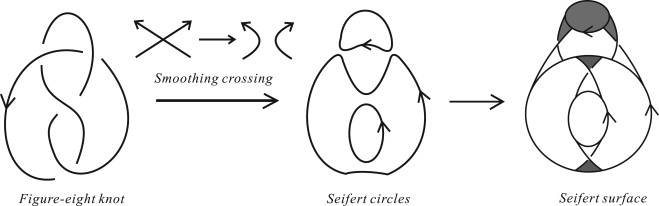
\includegraphics[width=0.75\textwidth]{../data/seifert-algorithm.jpg}
        \caption[Smthing]{Kolejne kroki algorytmu Seiferta}
    \end{figure}

    Dyski są dwustronne, więc ich górnej stronie przypisujemy znak $+$,
    jeśli tylko brzeg jest zorientowany dodatnio i~$-$ w~przeciwnym razie.
\index{algorytm!Seiferta|)}%
\end{proof}

Powierzchnia Seiferta dziedziczy orientację po węźle.
Nawet niewinne odwrócenie jednego z ogniw splotu potrafi istotnie zmienić jego powierzchnię, dlatego potrzebna jest ostrożność!

\index{powierzchnia!Seiferta|)}%

% Węzeł jest rozwłókniony dokładnie wtedy, gdy stanowi grzbiet pewnego 'open book decomposition' $S^3$.




\subsection{Węzły rozwłóknione}
\index{węzeł!włóknisty|see {węzeł rozwłókniony}}%
\index{węzeł!rozwłókniony|(}%
Wspomnijmy jeszcze krótko o~specjalnym rodzaju węzłów i splotów (patrz \cite[s. 49-50]{kawauchi96}).

% DICTIONARY;fibered;rozwłókniony, włóknisty;-
\begin{definition}
    Niech $L \subseteq S^3$ będzie splotem.
    Jeśli istnieje rodzina $F_t$ powierzchni Seiferta dla splotu $K$ sparametryzowana przez $t \in S^1$ taka, że $F_t \cap F_s = K$ dla $t \neq s$, to splot $K$ nazywamy rozwłóknionym albo włóknistym.
\end{definition}

\index{splot!Neuwirtha}%
Dawniej nazywano je splotami Neuwirtha, gdyż ten pokazał w~swojej pracy dyplomowej z~1959 roku, że można je scharakteryzować jako sploty, których komutant grupy podstawowej jest skończenie generowany, lub równoważnie, wolny.

\begin{example}
    Niewęzeł, trójlistnik $3_1$, ósemka $4_1$, $5_{1}$, $6_{2}$, $6_{3}$, $7_{1}$, $7_{6}$, $7_{7}$, $8_{2}$, $8_{5}$, $8_{7}$, $8_{9}$, $8_{10}$, $8_{12}$, $8_{16}$..$8_{21}$, splot Hopfa oraz wszystkie węzły torusowe są rozwłóknione.
\end{example}

(Jeśli węzeł pierwszy o co najwyżej ośmiu skrzyżowaniach nie został wymieniony w tym przykładzie, to nie jest rozwłókniony).
Rozkład liczby węzłów rozwłóknionych wśród węzłów pierwszych wygląda następująco:
\begin{itemize}
\item 9 skrzyżowań -- 23 węzły,
\item 10 skrzyżowań -- 74 węzły,
\item 11 skrzyżowań -- 256 węzłów,
\item 12 skrzyżowań -- 873 węzły.
\end{itemize}
% ZWERYFIKOWANO: funkcja count_fibered

Lwia część analizy węzłów o 12 skrzyżowaniach została wykonana przez Stojmenowa i~Hirasawę, jak podaje baza danych KnotInfo \cite{knotinfo22}.
% źródło: https://knotinfo.math.indiana.edu/descriptions/fibered.html
\index[persons]{Hirasawa, Mikami}%
\index[persons]{Stojmenow, Aleksander}%

\begin{proposition}
\index{wielomian!Alexandera}%
    Pierwszy i~ostatni współczynnik wielomianu Alexandera węzła rozwłóknionego to $\pm 1$.
\end{proposition}

% Kryterium to jest wystarczające dla węzłów pierwszych o co najwyżej 10 skrzyżowaniach oraz alternujących, ale znany jest przykład niewłóknistego węzła o 21 skrzyżowaniach, którego wielomian Alexandera ma postać $t^4 - t^3 + t^2 - t +1$.
% TODO: ustalić, czemu tak dużo skrzyżowań (z której książki ten fakt?). Sam wynik wydaje się być folklorem, tzn. nie wiadomo kto pierwszy to pokazał.

Kryterium to jest wystarczające dla węzłów pierwszych o co najwyżej 10 skrzyżowaniach, ale $11n_{34}$, $11n_{42}$, $11n_{73}$ oraz osiemnaście węzłów pierwszych o 12 skrzyżowaniach nie są rozwłóknione mimo tego, jak wygląda ich wielomian Alexandera.
% ZWERYFIKOWANO: funkcja alexander_fibered

\begin{example}
\index{węzeł!skręcony}%
    Niech $K$ będzie węzłem skręconym z $n$ półskrętami.
\index{wielomian!Alexandera}%
    Wtedy jego wielomianem Alexandera jest
    \begin{equation}
        \alexander_n(t) = n \cdot \left(t + \frac 1 t \right) - (2n+1),
    \end{equation}
    więc węzeł $K$ nie jest rozwłókniony, chyba że $n = 1$.
\end{example}

\begin{corollary}
% TODO: węzeł dokerski do indeksu?
    $2$-skręcony węzeł $6_1$ (węzeł dokerski) nie jest rozwłókniony.
\end{corollary}

Rolfsen \cite[s. 326]{rolfsen76} podaje jako ćwiczenie w swojej książce:

\begin{proposition}
\index{suma spójna}%
    Rodzina węzłów rozwłóknionych jest zamknięta na branie sum spójnych.
\end{proposition}

Dzięki książce Kawauchiego \cite[s. 84]{kawauchi96} wiem jeszcze, że Stallings ma swoje twierdzenie o~rozwłóknienieach dla zwartych 3-rozmaitości ze specjalnym przypadkiem:

\begin{proposition}
    Niech $y$ będzie jedynym epimorfizmem grupy splotu $L$ na nieskończoną grupę cykliczną $\langle t \rangle$, który posyła każdy południk na $t$. % each meridian
    Wtedy splot $L$ jest rozwłókniony wtedy i tylko wtedy, gdy jądro $\ker y$ jest skończenie generowalne.
\end{proposition}

\index{węzeł!rozwłókniony|)}%

% koniec podsekcji Węzły rozwłóknione




\subsection{Genus}
\index{genus|(}%
%label{sec:genus}%
Zanim przejdziemy do zdefiniowania macierzy Seiferta, potrzebować będziemy krótkiego skoku w bok -- zrozumieć bardzo geometryczny niezmiennik węzłów, genus.

Zaczniemy od starego twierdzenia, które klasyfikuje powierzchnie domknięte.

\begin{proposition}
    Każda powierzchnia domknięta jest członkiem jednej z dwóch nieskończonych rodzin:
    \begin{enumerate}[leftmargin=*]
        \itemsep0em
        \item sumą spójną $g \ge 0$ torusów,
        \item sumą spójną $k \ge 1$ rzeczywistych płaszczyzn rzutowych.
    \end{enumerate}
\end{proposition}

Elementy pierwszej rodziny są orientowalne.
Sferę traktujemy dla wygody jako sumę spójną $g = 0$ torusów.
Wtedy sumę spójną $g$ torusów możemy wyobrazić sobie jako sferę, do której doklejono $g$ uchwytów.

\begin{definition}[genus powierzchni]
    Ilość torusów nazywamy genusem powierzchni i oznaczamy literą $\genus$.
\end{definition}

Podobna charakteryzacja istnieje dla powierzchni z~brzegiem.
Każdy taki obiekt jest homeomorficzny z~sumą spójną $g$ torusów, w~których wydrążono pewną liczbę otworów: tyle, ile składowych spójności ma brzeg powierzchni.
W~przypadku powierzchni Seiferta mamy do czynienia z jednym otworem.

Dla wygody przypomnijmy jeszcze definicję klasycznego niezmiennika powierzchni:

\begin{definition}[charakterystyka Eulera]
\index{charakterystyka Eulera}%
    Niech $M$ będzie domkniętą powierzchnią orientowalną.
    Po striangulowaniu, składa się z $k_0$ wierzchołków, $k_1$ krawędzi oraz $k_2$ ścian.
    Wielkość
    \begin{equation}
        \chi = k_0 - k_1 + k_2
    \end{equation}
    jest niezmiennikiem powierzchni, zwanym charakterystyką Eulera.
\end{definition}

Definicja ta nie jest wygodna podczas ręcznych obliczeń.
Mamy za to:

\begin{proposition}
    Charakterystykę Eulera powierzchni jednoznacznie wyznaczają cztery reguły:
    \begin{itemize}
        \item jeśli $M$ jest dyskiem, to $\chi(M) = 1$,
        \item jeśli $M_1, M_2$ są powierzchniami, to $\chi(M_1 \sqcup M_2) = \chi(M_1) + \chi(M_2)$,
        \item jeśli powierzchnia $M_2$ powstaje z $M_1$ przez dołączenie paska, to $\chi(M_2) = \chi(M_1) - 1$,
        \item jeśli powierzchnia $M_2$ powstaje z $M_1$ przez dołączenie dysku do całej składowej spójności brzegu, to $\chi(M_2) = \chi(M_1) + 1$.
    \end{itemize}
\end{proposition}

Genus oraz charakterystyka Eulera są ze sobą związane:

\begin{proposition}
    Niech $M$ będzie powierzchnią o genusie $\genus$ i $\mu$ składowych spójności brzegu.
    Wtedy
    \begin{equation}
        \chi = 2 - \mu - 2\genus.
    \end{equation}
\end{proposition}

Nas interesują głównie powierzchnie Seiferta węzłów:
\index{powierzchnia Seiferta}%

\begin{proposition}
\label{prp:seifert_euler_characteristics}%
    Niech $K$ będzie węzłem z~diagramem $D$.
    Wtedy $\chi(M_D) = d - b$, gdzie $b$ jest liczbą skrzyżowań $D$, zaś $d$ jest liczbą okręgów Seiferta.
\end{proposition}

Można przeczytać o tym w \cite[s. 82]{murasugi96}.

\begin{proof}
    W~dowodzie faktu \ref{prp:seifert_exists} widzieliśmy, że liczba skrzyżowań $b$ jest jednocześnie liczbą pasków doklejonych do dysków.
    Bezpośredni rachunek pokazuje, że wtedy $k_0 = 4b$, $k_1 = 6b$ oraz $k_2 = b+d$.
    Wynika stąd, że $\chi = 4b - 6b + b + d = d - b$.
\end{proof}

Reszta tej podsekcji nie jest wymagana do zrozumienia macierzy Seiferta, przyjrzymy się genusowi jako obiektowi ciekawemu samemu w sobie.

\begin{definition}[3-genus]
    Niech $K$ będzie węzłem.
    Wśród wszystkich powierzchni Seiferta węzła $K$ istnieje co najmniej jedna o minimalnym genusie, jej genus nazywamy 3-genusem węzła $K$ i oznaczamy także przez $\genus$.
\end{definition}

Jeżeli nie powoduje to nieporozumień, zamiast 3-genus można pisać po prostu genus.

\begin{proposition}
\label{prp:genus_detects_unknot}%
    Genus wykrywa niewęzły: $K$ jest niewęzłem wtedy i tylko wtedy, gdy $g(K) = 0$.
\end{proposition}

\begin{proof}
    Niech $K$ będzie węzłem o genusie $0$.
    Z~charakteryzacji powierzchni wynika, że jego powierzchnia Seiferta to suma spójna $0$ torusów, to znaczy kula z tyloma otworami, ile $K$ ma ogniw.
    Innymi słowy, powierzchnią Seiferta węzła $K$ jest dysk, którego brzeg stanowi niewęzeł.
    To pokazuje, że implikacja w lewo jest prawdziwa.

    Implikacja w prawo jest oczywista.
\end{proof}

\subsubsection{Ograniczanie genusu z dołu}
Znalezienie 3-genusu dowolnego węzła sprawia te same trudności, co wyznaczenie jego liczby gordyjskiej.
Dowolna powierzchnia Seiferta zadaje ograniczenie z góry.
Z dołu 3-genus można szacować przy użyciu wielomianu Alexandera:
\index{wielomian!Alexandera}%

\begin{proposition}
\label{prp:alexander_genus}%
    Niech $K$ będzie węzłem.
    Wtedy $\operatorname{span} \alexander_K(t) \le 2\genus(K)$.
\end{proposition}

Fakt ten znalazłem w podręczniku Murasugiego \cite[s. 131]{murasugi96}.

\begin{proof}
    Załóżmy, że $F$ jest powierzchnią Seiferta węzła $K$ o genusie $g$.
    Wtedy macierz Seiferta powstała z $F$ jest stopnia $2g$, więc żaden ze składników jej wyznacznika nie może mieć stopnia (jako wielomian) większego niż $2g$.
\end{proof}

To dolne ograniczenie jest realizowane przez pewną powierzchnię Seiferta dla każdego pierwszego węzła o~co najwyżej 11 skrzyżowaniach poza siedmioma wyjątkami: 11n42, 11n67, 11n97 ($g = 2$), 11n34, 11n45, 11n73 oraz 11n152 ($g = 3$).
% warto byłoby dodać jakiś kod pozwalający sprawdzić, czemu akurat te węzły

\begin{proposition}
    Niech $K$ będzie węzłem, zaś $M$ jego macierzą Seiferta.
    Równość $\operatorname{span} \alexander_K(t) = 2\genus(K)$ zachodzi wtedy i tylko wtedy, gdy wyznacznik $\det M \neq 0$ jest niezerowy.
\end{proposition}

Floer zdefiniował w~\cite{floer90} przestrzeń wektorową nazywaną teraz homologią Floera, jest ona wyposażona w~endomorfizm parzystego stopnia, który powstaje z 2-wymiarowej klasy homologii reprezentowanej przez powierzchnię Seiferta.
%~kanoniczną gradację modulo $2$ oraz
\index{homologia!Floera}
Ta homologia rozkłada się na sumę prostą przestrzeni własnych wyróżnionego endomorfizmu, ich charakterystyki Eulera są współczynnikami wielomianu Alexandera.
Pozwala to na dokładniejsze szacowanie genusu węzła, patrz prace Ozsvátha, Szabó \cite{szabo03} i Ghigginiego \cite{ghiggini08}.
\index[persons]{Ghiggini, ?}%
\index[persons]{Ozsváth, Peter}%
\index[persons]{Szabó, Zoltán}%

\subsubsection{Ograniczanie genusu z góry}
Z góry genus ograniczony jest przez kilka klasycznych niezmienników numerycznych.
Zanim to pokażemy, przytoczymy techniczny lemat udowodniony przez Yamadę (\cite{yamada87}):
\index[persons]{Yamada, Shuji}%
% Morton MathSciNet: "The proof uses an ingenious direct algorithm to alter the projection without changing the number of Seifert circles"

\begin{proposition}
    \label{prp:seifert_circles_braid}
    Niech $L$ będzie splotem, zaś $\operatorname{s} L$ minimalną liczbą okręgów Seiferta, które dostajemy ze wszystkich możliwych diagramów splotu $L$.
    Wtedy $\operatorname{s} L = \braid L$ jest równe indeksowi warkoczowemu.
\index{indeks warkoczowy}%
\end{proposition}

Powyższe stwierdzenie występuje bez dowodu (bez?) w \cite[s. 17]{kawauchi96}.

\begin{proposition}
    Niech $L$ będzie splotem.
    Wtedy $\crossing L - \braid L - \operatorname{\mu} L + 2 \ge 2 \genus L$.
\end{proposition}

\begin{proof}
    Ustalmy minimalny diagram $D$ dla splotu $L$ i zastosujmy do niego algorytm Seiferta.
    Dostaniemy tak $s$ okręgów Seiferta oraz powierzchnię o genusie $g$.
    Fakt \ref{prp:seifert_euler_characteristics} mówiący, że $\chi = s - c$, można przekształcić do
    \begin{equation}
        g = \frac{c + 2 - s - \mu(K)}{2}.
    \end{equation}
    Z~minimalności diagramu wynika, że $c = \crossing L$.
    Fakt \ref{prp:seifert_circles_braid} mówi, że $s \ge \braid L$.
    Nierówność $g \ge \genus L$ wynika z~definicji genusu.
    Z powyższych rozważań wynika, że
    \begin{equation}
        \crossing L + 2 \ge 2 \genus L + \braid L + \operatorname{\mu} L,
    \end{equation}
    a to jest równoważnie nierówności, której prawdziwości dowodzimy.
\end{proof}

\begin{corollary}
    \label{cor:crossing_genus}
    Niech $K$ będzie węzłem.
    Wtedy $\crossing K \ge 2 \genus K$.
\index{indeks skrzyżowaniowy}
\end{corollary}

\subsubsection{Genus a rozkład na sumę węzłów pierwszych}

\begin{proposition}
    \label{prp:genus_of_sum}
    Jeśli $J, K$ są węzłami, to $g (J \shrap K) = g(J) + g(K)$.
\end{proposition}

Poniższy dowód pochodzi od Schuberta (\cite{schubert49}), został tylko zapisany we współczesnym języku.
\index[persons]{Schubert, Horst}%
Przebiega w dwóch etapach: najpierw pokazuje się, że genus sumy nie jest większy od sumy genusów składników, a następnie, że nie jest od niej mniejszy.

\begin{proof}
    Pokażemy najpierw, że $g(J \# K) \le g(J) + g(K)$.
    Wybierzmy powierzchnie Seiferta $M_J$ oraz $M_K$ dla $J$ oraz $K$ o~minimalnym genusie.
    Suma $J \shrap K$ powstaje z~$J$ oraz $K$, podobnie jest z~powierzchniami Seiferta:
\begin{comment}
    \begin{figure}[H]
        \centering
        \begin{minipage}[b]{.48\linewidth}
        \[
            \LargeGenusProofA \longrightarrow \LargeGenusProofB
        \]
        \subcaption{suma węzłów}
        %
        \end{minipage}
        \begin{minipage}[b]{.48\linewidth}
        \[
            \LargeGenusProofC \longrightarrow \LargeGenusProofD
        \]
        \subcaption{suma powierzchni}
        \end{minipage}
    \end{figure}
\end{comment}

    Skoro $M_{J\#K}$ powstaje z~$M_J \sqcup M_K$ przez dołączenie paska do brzegu, mamy
    \begin{equation}
        \chi(M_{J\#K}) = \chi(M_J \sqcup M_K) - 1 = \chi(M_J) + \chi(M_K)-1,
    \end{equation}
    a~przez to
    \begin{equation}
        g(M_{J\#K}) = \frac{1-\chi(M_{J\#K})}{2} =
        \frac{1-\chi(M_{J})}{2} + \frac{1-\chi(M_{K})}{2}
        % = %g(M_J)+g(M_K)
        = g(J) + g(K).
    \end{equation}
    To kończy dowód pierwszej nierówności.
    Pokażemy jeszcze, że $g(J \# K) \ge g(J)+g(K)$.
    Zaczynamy od powierzchni Seiferta $M_{J\#K}$ dla $J\#K$ o~minimalnym genusie $g(M_{J\#K})$ równym $g(J\#K)$.
    Poprzez wykonanie chirurgii na powierzchni, możemy przyjąć specjalną postać jak w~poprzednim dowodzie:
\begin{comment}
    \[
        \LargeGenusProofD
    \]
\end{comment}

    Usunięcie paska daje powierzchnie Seiferta dla $M_J$ oraz $M_K$ takie, że
    \begin{equation}
        g(M_J)+g(M_K)=g(M_{J\#K})=g(J\#K).
    \end{equation}
    Oznacza to, że $g(J) + g(K) \le g(M_J) + g(M_K) = g(J\#K)$ i~mamy równość.
\end{proof}

Jesteśmy wreszcie w~stanie podać prawdziwy dowód faktu \ref{first_time_sum_is_trivial}.

\begin{corollary}
    \label{cor:connected_sum_no_inverses}
    Jeśli suma spójna dwóch węzłów jest niewęzłem, to oba składniki także nim są.
\end{corollary}

Powrócimy teraz do węzłów pierwszych.
\index{węzeł!pierwszy}%

\begin{proposition}
    Niech $K$ będzie węzłem.
    Jeśli $g(K) = 1$, to $K$ jest węzłem pierwszym.
\end{proposition}

\begin{proof}
    Załóżmy nie wprost, że węzeł $K = K_1 \# K_2$ jest sumą dwóch nietrywialnych węzłów.
    Z~faktu \ref{prp:genus_of_sum} wynika wtedy, że $g(K) = g(K_1) + g(K_2)$.
    Zatem jeden z węzłów $K_1, K_2$ ma genus zero i jest trywialny, wbrew naszemu założeniu.
\end{proof}

Implikacja odwrotna jest fałszywa: pięciolistnik jest pierwszy, ale jego genus wynosi $2$.

\begin{proposition}
    Każdy węzeł można zapisać jako suma spójna pewnej liczby węzłów pierwszych.
    Niewęzeł jest sumą pustej rodziny węzłów.
\end{proposition}

\begin{proof}
    Dowodzimy przez indukcję względem genusu $g(K)$.
    Przypadek bazowy $g(K) = 0$ jest oczywisty, gdyż wtedy $K$ to niewęzeł.
    Załóżmy więc, że fakt zachodzi dla węzłów $J$ genusu co najwyżej $n$.
    Niech $K$ będzie genusu $n + 1$.

    Jeśli $K$ jest pierwszy, nie ma czego dowodzić.
    W przeciwnym razie jest równoważny z~$J_1 \shrap J_2$, gdzie $J_1$ i~$J_2$ są nietrywialne.
    Mamy $g(J_1) + g(J_2) = g(K)$ oraz $g(J_1),g(J_2) \ge 1$.
    Zatem $g(J_1), g(J_2) \le n$.
    Na mocy hipotezy indukcyjnej, $J_1$ oraz $J_2$ są równoważne sumom
    \[
        J_1 \cong K_1\#\cdots\# K_s,\qquad
        J_2 \cong K_{s+1}\#\cdots\# K_r,
    \]
    gdzie $K_i$ są pierwsze.
    Zatem $K$ jest równoważny z~$K_1\#\cdots\# K_r$, co kończy dowód.
\end{proof}

Nasz aparat matematyczny jest niedostatecznie rozwinięty, by móc udowodnić jedyność rozkładu.

\begin{theorem}[Schubert, 1949]
    Każdy nietrywialny węzeł rozkłada się na węzły pierwsze.
    Rozkład jest, z dokładnością do kolejności składników, jednoznaczny.
\index{węzeł!pierwszy}%
\end{theorem}

Schubert podał geometryczny dowód oparty o powierzchnie Seiferta; wyraził go w języku PL-rozmaitości (\cite{schubert49}), ale niedużym wysiłkiem można dokonać adaptacji do gładkiego świata.
\index[persons]{Schubert, Horst}%
Praca Schuberta korzysta z twierdzenia Alexandera, że 2-sfera w przestrzeni $\R^3$ ogranicza dysk, i jego odpowiednika dla torusów w $S^3$.

Hashizume \cite{hashizume58} rozszeszył wyniki Schuberta do splotów.
\index[persons]{Hashizume, ?}%
% trzeba wspomnieć, że to wymaga adaptacji definicji sumy spójnej, bo wcześniej dopuszczaliśmy tylko węzły jako składniki. Remedium = Kawauchi.

\begin{proposition}
    \label{prp:infinitely_many_prime_knots}
    Istnieje nieskończenie wiele węzłów pierwszych.
\end{proposition}

\begin{proof}
    Pokażemy, że wszystkie węzły $(2n+2)_1$ są pierwsze, gdzie $n \ge 1$.
    Istotnie, algorytm Seiferta zastosowany do diagramu tego węzła wyprodukuje $2n+1$ okręgów.
\begin{comment}
    \[
        \begin{tikzpicture}[baseline=-0.65ex,scale=0.06]
        \begin{knot}[clip width=7, flip crossing/.list={1,4,5},end tolerance=1pt]
            \node at (0,10) {$\cdots$};
            \strand[semithick] (-30, -5) -- (-5, -5);
            \strand[semithick]  (5, -5) -- (30, -5);
            \strand[semithick,latex-]  (-30,-15) -- (-5,-15);
            \strand[semithick]  (5,-15) -- (30,-15);

            \strand[semithick] (-5, -15) [in=down, out=right] to (5, -10) [in=right, out=up] to (-5, -5);
            \strand[semithick] (5, -15) [in=down, out=left] to (-5, -10) [in=left, out=up] to (5, -5);

            % zewnętrzne obręcze -- lewa strona
            \strand[semithick] (-30, 15) to [out=left, in=up]   (-45, 0);
            \strand[semithick] (-30,-15) to [out=left, in=down] (-45, 0);
            \strand[semithick] (-30,  5) to [out=left, in=up]   (-35, 0);
            \strand[semithick] (-30, -5) to [out=left, in=down] (-35, 0);

            % zewnętrzne obręcze -- prawastrona
            \strand[semithick] (30, 15) to [out=right, in=up]   (45,0);
            \strand[semithick] (30,-15) to [out=right, in=down] (45,0);
            \strand[semithick] (30,  5) to [out=right, in=up]   (35,0);
            \strand[semithick] (30, -5) to [out=right, in=down] (35,0);

            % jak w~drugim ruchu Reidemeistera - górny warkocz, lewy
            \strand[semithick] (-30, 15) [in=left, out=right] to (-20,  5);
            \strand[semithick] (-30,  5) [in=left, out=right] to (-20, 15);
            \strand[semithick] (-10, 15) [in=right, out=left] to (-20,  5);
            \strand[semithick] (-10,  5) [in=right, out=left] to (-20, 15);

            % jak w~drugim ruchu Reidemeistera - górny warkocz, prawy
            \strand[semithick] (30, 15) [in=right, out=left] to (20,  5);
            \strand[semithick] (10, 15) [in=left, out=right] to (20,  5);
            \strand[semithick] (30,  5) [in=right, out=left] to (20, 15);
            \strand[semithick] (10,  5) [in=left, out=right] to (20, 15);
        \end{knot}
        \end{tikzpicture}
        \longrightarrow
        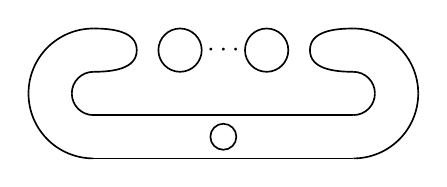
\begin{tikzpicture}[baseline=-0.65ex,scale=0.055]
            \node at (0,10) {$\cdots$};
            \draw[semithick] (-30,  -5) -- (30, -5);
            \draw[semithick] (-30, -15) -- (30,-15);

            \draw[semithick] (0,-10) circle (3);

                % zewnętrzne obręcze -- lewa strona
            \draw[semithick] (-30, 15) to [out=left, in=up]   (-45, 0);
            \draw[semithick] (-30,-15) to [out=left, in=down] (-45, 0);
            \draw[semithick] (-30,  5) to [out=left, in=up]   (-35, 0);
            \draw[semithick] (-30, -5) to [out=left, in=down] (-35, 0);

                % zewnętrzne obręcze -- prawastrona
            \draw[semithick] (30, 15) to [out=right, in=up]   (45,0);
            \draw[semithick] (30,-15) to [out=right, in=down] (45,0);
            \draw[semithick] (30,  5) to [out=right, in=up]   (35,0);
            \draw[semithick] (30, -5) to [out=right, in=down] (35,0);

            \draw[semithick] (-30, 15) to [out=right, in=up] (-20,10);
            \draw[semithick] (-30,  5) to [out=right, in=down] (-20,10);

            \draw[semithick] (30, 15) to [out=left, in=up] (20,10);
            \draw[semithick] (30,  5) to [out=left, in=down] (20,10);

            \draw[semithick] (-10, 10) circle (5);
            \draw[semithick] (10,  10) circle (5);
        \end{tikzpicture}
    \]
\end{comment}
    Wynika stąd, że genus wynosi $\frac 12 (1 - (1+2n) + (2+2n)) = 1$, ponieważ wyznacznik ma wartość $4n+1$,
    węzły $(2n+2)_1$ nie są trywialne i~są parami różne.
\end{proof}

\subsubsection{Genus kanoniczny, genus wolny}
% DICTIONARY;free;wolny;genus
% DICTIONARY;canonical;kanoniczny;genus
% DICTIONARY;genus;genus;-
Czy w definicji genusu można ograniczyć się do tych powierzchni Seiferta, które pochodzą od algorytmu Seiferta?
Niestety, poza pewnymi wyjątkami, nie.
Zanim przekonamy się, dlaczego tak jest, zdefiniujmy jeszcze dwa niezmienniki.

\begin{definition}[genus kanoniczny]
\index{genus!kanoniczny}%
    Niech $K$ będzie węzłem.
    Najmniejszy z genusów powierzchni Seiferta węzła $K$, które pochodzą z~algorytmu Seiferta, nazywamy genusem klasycznym i~oznaczamy symbolem $\operatorname{g_c} K$ lub krótko $g_c$.
\end{definition}

Stojmenow \cite{stoimenow08} opisał diagramy węzłów o~kanonicznym genusie równym 2.
\index[persons]{Stojmenow, Aleksander}%
Część z~jego wyników przenosi się na genus 3.
Jak sam pisze, sklasyfikowane wcześniej węzły o~genusie (kanonicznym) 1 okazały się być zbyt wąską klasą.

Pod koniec lat pięćdziesiątych Crowell i~Murasugi niezależnie zauważyli, że algorytm Seiferta zastosowany do alternującego diagramu zawsze daje powierzchnię o~minimalnej powierzchni.
\index[persons]{Crowell, ?}%
\index[persons]{Murasugi, Kunio}%
Ich kombinatoryczne uzasadnienie było dość zawiłe, elementarny dowód podał Gabai w \cite{gabai86}.
\index[persons]{Gabai, David}%

Dubel trójlistnika ma genus równy $1$, ale algorytm Seiferta zastosowany wobec węzła produkuje powierzchnie o genusie co najmniej $3$, jak przewiduje ograniczenie znalezione przez Mortona w \cite[twierdzenie 2]{morton86}:

\begin{proposition}
    Niech $P(v, z)$ będzie wersją wielomianu HOMFLY spełniającą zależność
    \begin{equation}
        \frac 1v P_+ - vP_- = zP_0.
    \end{equation}
    Wtedy $M = \max \deg_z P(v, z) \le 2g_c$.
\end{proposition}

Nierówność Mortona jest równością dla wielu klas węzłów, w tym
\index{nierówność Mortona}%
alternujących (Crowell, Murasugi),
\index[persons]{Crowell, ?}%
\index[persons]{Murasugi, Kunio}%
\index{węzeł!alternujący}%
jednorodnych\footnote{Uogólnienie węzłów alternujących.} (Cromwell w \cite{cromwell89}),
\index{węzeł!jednorodny}%
\index[persons]{Cromwell, Peter}%
whiteheadowskich dubli węzłów dwumostowych (Nakamura w \cite{nakamura06}, Tripp w \cite{tripp02}) albo
\index{dubel Whiteheada}%
\index{węzeł!dwumostowy}%
\index[persons]{Nakamura, Takuji}%
\index[persons]{Tripp, ?}%
precli (Brittenham, Jensen \cite{brittenham06}).
\index[persons]{Brittenham, ?}%
\index[persons]{Jensen, ?}%
\index{precel}%
Stojmenow pokazał, że staje się równością dla węzłów o co najwyżej 12 skrzyżowaniach i znalazł przykład węzła, dla którego jest ostra.
\index[persons]{Stoimenow, Alexander}%

\begin{definition}[genus wolny]
\index{ciało z rączkami}%
\index{genus!wolny}%
    Niech $K$ będzie węzłem.
    Minimalny genus spośród powierzchni Seiferta węzła $K$, których dopełnienie w 3-sferze jest ciałem z rączkami, nazywamy genusem wolnym i~oznaczamy $g_f$.
\end{definition}

Dopełnienie powierzchni Seiferta jest zawsze ciałem z rączkami, więc mamy oczywiste nierówności
\begin{equation}
    g \le g_f \le g_c.
\end{equation}
Jak duża może być różnica między kolejnymi genusami?
Już Kirby \cite[problem 1.20a]{kirby78} chciał znać oszacowania różnicy $g_f - g$.
Morton \cite{morton86} pokazał, że genus pewnych węzłów nie jest realizowany przez żaden diagram do którego stosuje się algorytm Seiferta, choćby $10_{165}$.
Moriah, matematyk izraelski, rozwiązał problem Kirby'ego dekadę później:

\begin{proposition}
    Niech $K$ będzie węzłem, $D_k(K)$ jego dublem Whiteheada z $k \neq 0$ skręceniami, zaś $B_n(K)$ to $n$-krotne nakrycie cykliczne sfery $S^3$ rozgałęzione nad węzłem $K$.
    Jeżeli ranga pierwszej grupy homologii $B_{|4k+1|}(K)$ wynosi $r$, to
    \begin{equation}
        g_f(D_k(K)) \ge \frac {2r-1} {|8k+2|}.
    \end{equation}
\end{proposition}

\begin{proof}
    Praca \cite{moriah87}.
    Dowód opiera się na chirurgii węzłów i splotów w sferze $S^3$.
\end{proof}

\begin{corollary}
    Niech $K$ bedzie sumą spójną $n$ trójlistników, połóżmy $k = -1$.
    Wtedy pierwsza grupa homologii ma rangę $r = 2n$ i~genus wolny jest nieograniczony
    \begin{equation}
        g_f(D_{-1}(3_1^n)) \ge \frac {4n-1} {6},
    \end{equation}
    podczas gdy zwykły genus to $g(D_{-1}(3_1^n)) = 1$.
\end{corollary}

Kawauchi \cite{kawauchi94} zbadał węzeł $K_m$, sumę spójną $m$ kopii skręconego whiteheadowskiego dubla trójlistnika, i policzył, że różnica $g_c(K_m) - g(K_m)$ wynosi $2m$.
Wreszcie Kobayashi oraz Kobayashi \cite{kobayashi96} wskazali nieskończoną rodzinę węzłów nieograniczonego genusu, dla której
\begin{equation}
    g_c(K) = \frac 32 g_f(K) = 2g(K).
\end{equation}
% znam ich ze Stojmenow - Knots of (canonical) genus two

\index{genus|)}

% Koniec podsekcji Genus




\subsection{Macierz Seiferta}
\index{macierz Seiferta|(}
Niech $K$ będzie węzłem z diagramem $D$ i powierzchnią Seiferta $S$.

% Murasugi, s. 79
\begin{definition}[graf Seiferta]
\index{graf Seiferta}%
    Ściągnijmy dyski z dowodu faktu \ref{prp:seifert_exists} do punktów jednocześnie kurcząc doklejone paski, otrzymamy graf zwany grafem Seiferta diagramu $D$.
\end{definition}

Murasugi \cite[s. 79]{murasugi96} proponuje jako ćwiczenie dowód faktu:

\begin{proposition}
    Graf Seiferta jest dwudzielny i planarny.
\end{proposition}

% Murasugi 82, 83
Skoro graf Seiferta jest planarny, to dzieli sferę $S^2$ na $f$ obszarów.
Można wyznaczyć ich liczbę: skoro $\chi(S^2) = d - b + f = 2$, to $f - 1 = 1 - d + b$, pomijamy obszar nieograniczony.
Brzeg każdego obszaru jest zamkniętą krzywą, z których tworzymy krzywe $x_1, \ldots, x_m$ na powierzchni Seiferta.
Generują one grupę podstawową $\pi_1(S)$.

Niech $S$ będzie powierzchnią Seiferta z wyróżnioną jedną stroną.
Jeśli krzywa $x_i$ biegnie po powierzchni $S$, przez $x_i^*$ oznaczać będziemy dodatnie wypchnięcie: krzywą równoległą do $x_i$, która biegnie tuż nad nią.
Potrzebowaliśmy wyróżnić jedną ze stron powierzchni $S$, by słowo ,,nad'' miało sens.

\begin{definition}[macierz Seiferta]
    Przy zachowaniu powyższych oznaczeń, macierz, której wyrazy określa wzór $M_{i,j} = \operatorname{lk}(x_i, x_j^*)$, nazywamy macierzą Seiferta.
\end{definition}

Konstrukcja macierzy Seiferta zależy od wyboru diagramu oraz orientacji krzywych $x_i$, dlatego nie jest niezmiennikiem węzłów.
Stanie się nim, kiedy uwzględnimy jeszcze wpływ ruchów Reidemeistera.

\begin{proposition}
    Kwadratowa macierz $V$ o całkowitych wyrazach jest macierzą Seiferta węzła wtedy i~tylko wtedy, gdy $\det(V - V^t) = 1$.
\end{proposition}

\begin{proof}
    Kawauchi \cite[s. 62]{kawauchi96} pisze, że wynika to z~klasyfikacji macierzy Seiferta splotów.
\end{proof}

\begin{definition}
    Operacja $\Lambda_1$ dla pewnej odwracalnej macierzy $P$ o całkowitych wyrazach (czyli $\det P = \pm 1$) to
    \begin{equation}
        \Lambda_1 \colon M \mapsto PMP^t.
    \end{equation}
    Natomiast operację $\Lambda_2$ definiuje wzór:
    \begin{equation}
        \Lambda_2 \colon M \mapsto \begin{bmatrix}
  &   &  & 0 & 0 \\
  & M &  & \vdots & \vdots \\
  &   &  & 0 & 0 \\
* & \dots & * & 0 & 0 \\
0 & \dots & 0 & 1 & 0
\end{bmatrix} \textrm{albo} \begin{bmatrix}
  &   &  & * & 0 \\
  & M &  & \vdots & \vdots \\
  &   &  & * & 0 \\
0 & \dots & 0 & 0 & 1 \\
0 & \dots & 0 & 0 & 0
\end{bmatrix},
    \end{equation}
    gdzie gwiazdka zastępuje ustaloną liczbę całkowitą.
\end{definition}

\begin{definition}
\index{S-równoważność}%
    Niech $M_1, M_2$ będą macierzami.
    Jeśli $M_2$ można otrzymać z $M_1$ przez skończony ciąg operacji $\Lambda_1, \Lambda_2$ oraz ich odwrotności, to macierze nazywamy $S$-równoważnymi.
\end{definition}

Badania powyższej relacji równoważności prowadzili w~latach sześćdziesiątych ubiegłego stulecia Trotter \cite{trotter62}, Murasugi \cite{murasugi65} oraz Levine \cite{levine70}.
\index{człowiek!Trotter, Hale}%
\index{człowiek!Murasugi, Kunio}%
\index{człowiek!Levine, Jerome}%
Litera $S$, jak nietrudno się domyślić, pochodzi od Seiferta.

\begin{proposition}
    Macierz Seiferta modulo $S$-równoważność jest niezmiennikiem splotów.
\end{proposition}

Dowód tego faktu jest elementarny, ale dość długi.
Razem z~ułatwiającymi zrozumienie diagramami można znaleźć go w podręczniku Murasugiego albo \cite[s. 64]{kawauchi96}, dlatego pomijamy go i skupimy się na tym, jakie niezmienniki można otrzymać z macierzy Seiferta.

Wyznacznik całej macierzy Seiferta nie jest niezmiennikiem.
Wykonując operację $\Lambda_2$ dostajemy macierz, której ostatnia kolumna albo ostatni wiersz są zerami, więc jej wyznacznik także jest zerem.
Jeśli jednak najpierw dokonamy jej symetryzacji, dostaniemy znany już niezmiennik.

\begin{proposition}
    Niech $M$ będzie macierzą Seiferta węzła $K$.
    Wtedy
    \begin{equation}
        \det K = |\det(M + M^t)|.
    \end{equation}
\end{proposition}

\index{wielomian!Alexandera}%
Przez wprowadzenie dodatkowej zmiennej $t \in \R$, ponownie uogólnimy wyznacznik do wielomianu Alexandera.

\begin{proposition}
    Niech $M$ będzie macierzą Seiferta stopnia $k$ węzła $K$.
    Wtedy
    \begin{equation}
        \alexander_K (t) = t^{-k/2}\det(M - tM^t).
    \end{equation}
\end{proposition}

Określimy jeszcze dwa, niewystępujący wcześniej niezmiennik (Arfa i sygnaturę).

\index{macierz Seiferta|)}




\subsection{Sygnatura}
\label{sub:signature}%
\index{sygnatura|(}%
Sygnatura jest kolejnym niezmiennikiem, do zdefiniowania których wystarczy znać macierz Seiferta.
Pochodzi prawdopodobnie z lat sześćdziesiątych (Trotter \cite{trotter62} dla węzłów, Murasugi \cite{murasugi65} dla splotów).
\index[persons]{Trotter, Hale}%
\index[persons]{Murasugi, Kunio}%
% z recenzji do 275415: Shinohara, Yaichi - On the signature of knots and links.
Ktoś powiedział nam kiedyś, że ujednolicenia różnych podejść do form kwadratowych związanych z węzłami dokonali Gordon, Litherland, Murasugi w~pracy \cite{litherland81}, ale potem trafiliśmy na artykuł Przytyckiego \cite{przytycki11} pełen historycznych ciekawostek oraz dwóch kolejnych odnośników: do wspomnianej przed chwilą pracy \cite{murasugi65}, ale też \cite{litherland78} samych Gordona, Litherlanda, którzy sięgają zenitu i wiążą dziełą Goeritza, Trottera, Murasugiego et alli.
Może po prostu najlepiej przeczytać wszystko?

% DICTIONARY;signature;sygnatura;-
\begin{definition}[sygnatura]
\label{def:signature}%
    Niech $M$ będzie macierzą Seiferta zorientowanego splotu $L$.
    Wielkość
    \begin{equation}
        \sigma_L := \operatorname{\sigma} (M + M^t),
    \end{equation}
    sygnaturę macierzy $M + M^t$, nazywamy sygnaturą splotu $L$.
\end{definition}

\begin{proposition}
\label{prp:signature_additive}%
    Sygnatura jest addytywna: $\sigma(K_1 \shrap \ldots \shrap K_n) = \sum_{k=1}^n \sigma(K_k)$.
\end{proposition}

Wiem o tym z \cite[s. 127]{murasugi96}.

\begin{proof}
    Bez straty ogólności ograniczmy się do przypadku $n = 2$ i~ustalmy powierzchnie Seiferta $F_1, F_2$ dla węzłów $K_1, K_2$ z~macierzami Seiferta $M_1, M_2$.
    Powierzchnia dla ich sumy spójnej $K_1 \shrap K_2$ powstaje przez sklejenie $F_1$ oraz $F_2$ paskiem.
    W języku macierzy oznacza to, że macierz Seiferta węzła $K_1 \shrap K_2$ ma postać $M = M_1 \oplus M_2$.
    Zatem:
    \begin{align}
        \sigma(K_1 \shrap K_2) & = \sigma(M + M^t) \\
                               & = \sigma(M_1 + M_1^t) + \sigma(M_2 + M_2^t) \\
                               & = \sigma(K_1) + \sigma(K_2),
    \end{align}
    co kończy dowód.
\end{proof}

\begin{corollary}
\index{liczba mostowa}%
\label{no_relation_signature_bridge}%
    Nie istnieje bezpośredni związek między sygnaturą i~liczbą mostową.
\end{corollary}

Patrz \cite[s. 145]{livingston93}.

\begin{proof}
    Węzeł torusowy $T_{2,n}$ jest dwumostowy, jego sygnatura wynosi $n - 1$.
    Suma spójna węzłów prostych (sumy przeciwnie zorientowanych trójlistników) ma zerową sygnaturę, ale na mocy faktu~\ref{prp:bridge_additive} jej liczba mostowa jest nieograniczona.
\end{proof}

\begin{proposition}
\index{lustro}%
\index{rewers}%
\label{prp:signature_mirror_reverse}%
    Niech $L$ będzie splotem.
    Wtedy $\sigma(mL) = -\sigma(L)$ oraz $\sigma(rL) = \sigma(L)$.
\end{proposition}

O tym także wiem z \cite[s. 127]{murasugi96}.

\begin{proof}
    Wynika to z podobnych faktów dla macierzy Seiferta.
    Równoważność $M_{mL} \simeq - M_L^t$ wynika z tego, że zamiana nad- i podskrzyżowań odwraca wzajemne położenie krzywych, których indeksu zaczepienia szukamy.

    Podobnie pokazuje się, że $M_{rL} \simeq M_L^t$.
\end{proof}

\begin{corollary}
\index{węzeł!achiralny}%
\label{cor:acheiral_signature}%
    Jeśli $K$ jest węzłem achiralnym, to $\sigma(K) = 0$.
\end{corollary}

Węzły achiralne mają zerową sygnaturę, zatem trójlistnik nie jest achiralny.
Z faktów~\ref{prp:signature_additive} oraz~\ref{prp:signature_mirror_reverse} wynika, że suma tak samo zorientowanych trójlistników nie jest achiralna ($\sigma = \pm 4$).
Jak można przekonać się ze standardowego diagramu węzła prostego, ten jest achiralny.
Pisaliśmy coś o tym na stronie \pageref{two_sums_of_two_trefoils}.

\begin{proposition}
\label{trivial_alexander_polynomial}%
\index{wielomian!Alexandera}%
    Niech $L$ będzie węzłem.
    Jeśli $\alexander_K(t) \equiv 1$, to $\sigma (K) = 0$.
\end{proposition}

Założenie $\alexander_K(t) \equiv 1$ jest spełnione przez cztery węzły pierwsze do 12 skrzyżowań, są to $11n_{34}, 11n_{42}, 12n_{313}$ oraz $12n_{430}$, patrz wzmianka po fakcie~\ref{alexander_no_detects_unknot}.
% ZWERYFIKOWANO: funkcja trivial_alexander

\begin{proof}
\index[persons]{Milnor, John}%
    Murasugi twierdzi, że zostało to udowodnione przez Milnora w \cite{milnor68}, nie jesteśmy jednak pewni, gdzie dokładnie, ale raczej poza sekcją piątą.
\end{proof}

Istnieje równoważna definicja, która nie wymaga czasochłonnego wyznaczania macierzy Seiferta.

\begin{proposition}
\index{relacja kłębiasta}%
    Sygnatura to niezmiennik topologiczny zadany kłębiastą relacją rekurencyjną:
    \begin{itemize}[leftmargin=*]
    \itemsep0em
        \item $\sigma (\SmallUnknot) = 0$,
        \item $\sigma (K_+) - \sigma (K_-) \in \{0, 2\}$,
        \item $4 \mid \sigma (K)$ wtedy i~tylko wtedy, gdy $\conway(2i) > 0$ (wielomian Conwaya).
    \end{itemize}
\end{proposition}

Symbole $K_+, K_-$ objaśnione są przy definicji~\ref{skein_symbols}.

\begin{proof}
    Wystarczy pokazać, że sygnatura węzła spełnia trzy powyższe aksjomaty, a~następnie zauważyć, że korzystając z~nich jesteśmy w~stanie wyznaczyć jednoznacznie sygnaturę dla dowolnego węzła.
    Wynika to z~faktu, że każdy węzeł można zmienić w~niewęzeł odwracając pewne skrzyżowania.
    Pomysł opisał dokładnie Giller \cite[trzecie spostrzeżenie]{giller82}, sam oparł się o~\cite[twierdzenie 5.6]{murasugi65}.
\index[persons]{Giller, Cole}%
\end{proof}

Sygnatura pozwala uzyskać proste oszacowanie liczby gordyjskiej od dołu:
\index{liczba gordyjska}%

\begin{proposition}
    Mamy $2 u(K) \ge |\sigma(K)|$.
\end{proposition}

Liczba gordyjska 83 z~801 węzłów pierwszych o mniej niż dwunastu skrzyżowaniach nie jest jeszcze znana.
Dla 272 spośród pozostałych mamy równość $2u = |\sigma|$.
% ZWERYFIKOWANO: funkcja unknotting_sigma 

\begin{proof}
    Ustalmy diagram $D$ dla węzła $K$.
    Odwrócenie dowolnego skrzyżowania polega na przejściu z~diagramu $D_+$ do $D_-$ lub z~$D_-$ do $D_+$.
    Zgodnie z relacją kłębiastą, sygnatura pozostaje taka sama lub zmienia wartość o $2$.
    Po wykonaniu $u$ odwróceń otrzymujemy diagram niewęzła o~sygnaturze zero, zatem sygnatura wyjściowego węzła nie mogła przekraczać $2u$.
    To kończy dowód.
\end{proof}

W~\cite{shinohara71} Shinohara pokazał, że dla każdej pary nieujemnych liczb całkowitych $m, n$ istnieje węzeł $K$ o wyznaczniku $4m+1$ ($8m+5$, $4m+3$) oraz sygnaturze bez znaku $8n$ ($8n+4$, $4n+2$).
\index[persons]{Shinohara, Yaichi}%
\index{wyznacznik}%
Ponadto, jeśli $m$ nie dzieli się przez $3$, istnieje węzeł o wyznaczniku $8m+1$ i sygnaturze bez znaku $8n+4$.
% skąd to? Ohtsuki?

Czas na raczej niezbyt użyteczną ciekawostkę.

\begin{conjecture}
    Czy istnieje węzeł o~sygnaturze $4$ i~wyznaczniku postaci $n = 4k + 1$?
\end{conjecture}

Stojmenow twierdzi, że jeśli tak jest, to wszystkie pierwsze dzielniki $n$ dają resztę $1$ z~dzielenia przez $24$ i~są większe od $2857$.
\index[persons]{Stojmenow, Aleksander}%
Patrz \cite[s. 540]{ohtsuki02}.

Czytając przeglądową pracę Conwaya \cite{conway19} dowiedzieliśmy się, że w~latach sześćdziesiątych sygnatura została uogólniona do funkcji $\sigma_L \colon S^1 \to \Z$.
\index[persons]{Conway, John}%
Większość podręczników, a także prace Levine'a \cite{levine69} oraz Tristrama \cite{tristram69}, wprowadza ją przy użyciu macierzy Seiferta, więc my postąpimy dokładnie tak samo.
\index[persons]{Levine, Jerome}%
\index[persons]{Tristram, Andrew}%

\begin{definition}[sygnatura Levine'a-Tristrama]
\index{sygnatura!Levine'a-Tristrama}%
    Niech $M$ będzie macierzą Seiferta zorientowanego splotu $L$.
    Funkcję $\sigma_L \colon S^1 \to \Z$ daną wzorem
    \begin{equation}
        \sigma_L(\omega) := \operatorname{\sigma} [(1-\omega) M + (1 - \overline{\omega})M^t]
    \end{equation}
    nazywamy sygnaturą Levine'a-Tristrama splotu $L$.
    Jest niezmiennikiem splotów.
\end{definition}

Funkcja $\sigma_L$ jest kawałkami stała.
Conway pisze w \cite{conway19}, że wynika to ze wzoru na wielomian Alexandera $\Delta_L(t) = \det(tM - M^t)$.
\index[persons]{Conway, John}%
\index{wielomian!Alexandera}%
Jedynymi punktami nieciągłości są zera wielomianu $(t-1)\Delta_L(t)$, to świeży wynik Gilmera, Livingstona z~\cite{gilmer16}.
\index[persons]{Gilmer, Patrick}%
\index[persons]{Livingston, Charles}%

Mówimy, że funkcja zdefiniowana na okręgu jest zbalansowana, jeżeli w każdym punkcie nieciągłości przyjmuje wartość równą średniej z~lewo- oraz prawostronnej granicy w tym punkcie.
Livingston podał pełną charakteryzację zbilansowanych sygnatur Levine'a-Tristrama dla węzłów, analogiczny problem dla splotów wydaje się być wciąż otwarty.

\begin{proposition}
\label{balanced_iff_four_conditions}%
    Funkcja zbalansowana $\sigma \colon S^1 \to \Z$ jest realizowana jako sygnatura pewnego węzła wtedy i tylko wtedy, gdy:
    \begin{enumerate}
        \item dla każdego $\omega \in S^1$ mamy $\sigma(\omega) = \sigma(\overline{\omega})$
        \item $\sigma(1) = 0$
        \item każda nieciągłość funkcji $\sigma$ jest miejscem zerowym wielomianu Alexandera węzła
        \item jeżeli argumenty $\omega_1, \omega_2$ są sprzężone w sensie Galois, to $\sigma(\omega_1) \equiv \sigma(\omega_2)$ modulo $2$.
    \end{enumerate}
\end{proposition}

\begin{proof}
    Livingston pisze w \cite{livingston18}, że dowód w prawą stronę jest dość dobrze znany, natomiast w lewo korzysta z~wyników Kondo \cite{kondo79} i Sakaiego \cite{sakai77}, że każdy wielomian Alexandera węzła jest realizowany przez węzeł 1-gordyjski oraz zachowania zbalansowanej sygnatury podczas odwracania skrzyżowania.
\end{proof}

(Nie każdy wielomian Kauffmana/HOMFLY jest realizowany przez węzły 1-gordyjskie, Kawauchi \cite[s. 151]{kawauchi96} wspomina na przykład, że $\unknotting K \ge \log_3 |Q(-1)|$.)

\begin{proposition}
\index{węzeł!satelitarny}%
    Niech $S$ będzie satelitą z towarzyszem $C$, wzorcem $P$ oraz indeksem zaczepenia $n$.
    Wtedy
    \begin{equation}
        \sigma_S(\omega) = \sigma_P(\omega) + \sigma_C(\omega^n).
    \end{equation}
\end{proposition}

\begin{proof}
    Szczególny przypadek $\omega = -1$ rozpatrywał wcześniej Shinohara w~\cite{shinohara71}.
\index[persons]{Shinohara, Yaichi}%
    Pełny dowód znajduje się w artykule \cite{litherland79} Litherlanda.
\index[persons]{Litherland, Richard}%
\end{proof}

Wreszcie:

\begin{proposition}
    Niech $L$ będzie splotem.
    Wtedy albo wielomian Alexandera $\Delta_L(t)$ jest tożsamościowo zerem, albo posiada co najmniej $|\sigma_L|$ zer, liczonych z krotnościami, na okręgu jednostkowym.
\end{proposition}

\begin{proof}
    Aneks w książce Liechtiego \cite{liechti16}, która nie wygląda na związaną z~teorią węzłów.
\end{proof}

\index{sygnatura|)}%

% Koniec podsekcji Sygnatura



% koniec sekcji Powierzchnie Seiferta